%!TeX root=../sensetop.tex
\chapter[Chapter \thechapter]{}
\lettrine[lraise=0.3]{A}{fter} some opposition, Marianne yielded to her sister's entreaties, and consented to go out with her and Mrs Jennings one morning for half an hour. She expressly conditioned, however, for paying no visits, and would do no more than accompany them to Gray's in Sackville Street, where Elinor was carrying on a negotiation for the exchange of a few old-fashioned jewels of her mother.

When they stopped at the door, Mrs Jennings recollected that there was a lady at the other end of the street on whom she ought to call; and as she had no business at Gray's, it was resolved, that while her young friends transacted theirs, she should pay her visit and return for them.

On ascending the stairs, the Miss Dashwoods found so many people before them in the room, that there was not a person at liberty to tend to their orders; and they were obliged to wait. All that could be done was, to sit down at that end of the counter which seemed to promise the quickest succession; one gentleman only was standing there, and it is probable that Elinor was not without hope of exciting his politeness to a quicker despatch. But the correctness of his eye, and the delicacy of his taste, proved to be beyond his politeness. He was giving orders for a toothpick-case for himself, and till its size, shape, and ornaments were determined, all of which, after examining and debating for a quarter of an hour over every toothpick-case in the shop, were finally arranged by his own inventive fancy, he had no leisure to bestow any other attention on the two ladies, than what was comprised in three or four very broad stares; a kind of notice which served to imprint on Elinor the remembrance of a person and face, of strong, natural, sterling insignificance, though adorned in the first style of fashion.

Marianne was spared from the troublesome feelings of contempt and resentment, on this impertinent examination of their features, and on the puppyism of his manner in deciding on all the different horrors of the different toothpick-cases presented to his inspection, by remaining unconscious of it all; for she was as well able to collect her thoughts within herself, and be as ignorant of what was passing around her, in Mr Gray's shop, as in her own bedroom.

At last the affair was decided. The ivory, the gold, and the pearls, all received their appointment, and the gentleman having named the last day on which his existence could be continued without the possession of the toothpick-case, drew on his gloves with leisurely care, and bestowing another glance on the Miss Dashwoods, but such a one as seemed rather to demand than express admiration, walked off with a happy air of real conceit and affected indifference.

Elinor lost no time in bringing her business forward, was on the point of concluding it, when another gentleman presented himself at her side. She turned her eyes towards his face, and found him with some surprise to be her brother.

Their affection and pleasure in meeting was just enough to make a very creditable appearance in Mr Gray's shop. John Dashwood was really far from being sorry to see his sisters again; it rather gave them satisfaction; and his inquiries after their mother were respectful and attentive.

Elinor found that he and Fanny had been in town two days.

<I wished very much to call upon you yesterday,> said he, <but it was impossible, for we were obliged to take Harry to see the wild beasts at Exeter Exchange; and we spent the rest of the day with Mrs Ferrars. Harry was vastly pleased. \textit{This} morning I had fully intended to call on you, if I could possibly find a spare half hour, but one has always so much to do on first coming to town. I am come here to bespeak Fanny a seal. But tomorrow I think I shall certainly be able to call in Berkeley Street, and be introduced to your friend Mrs Jennings. I understand she is a woman of very good fortune. And the Middletons too, you must introduce me to \textit{them}. As my mother-in-law's relations, I shall be happy to show them every respect. They are excellent neighbours to you in the country, I understand.>

<Excellent indeed. Their attention to our comfort, their friendliness in every particular, is more than I can express.>

<I am extremely glad to hear it, upon my word; extremely glad indeed. But so it ought to be; they are people of large fortune, they are related to you, and every civility and accommodation that can serve to make your situation pleasant might be reasonably expected. And so you are most comfortably settled in your little cottage and want for nothing! Edward brought us a most charming account of the place: the most complete thing of its kind, he said, that ever was, and you all seemed to enjoy it beyond any thing. It was a great satisfaction to us to hear it, I assure you.>

Elinor did feel a little ashamed of her brother; and was not sorry to be spared the necessity of answering him, by the arrival of Mrs Jennings's servant, who came to tell her that his mistress waited for them at the door.

Mr Dashwood attended them down stairs, was introduced to Mrs Jennings at the door of her carriage, and repeating his hope of being able to call on them the next day, took leave.

\begin{figure}[tbph]
\centering
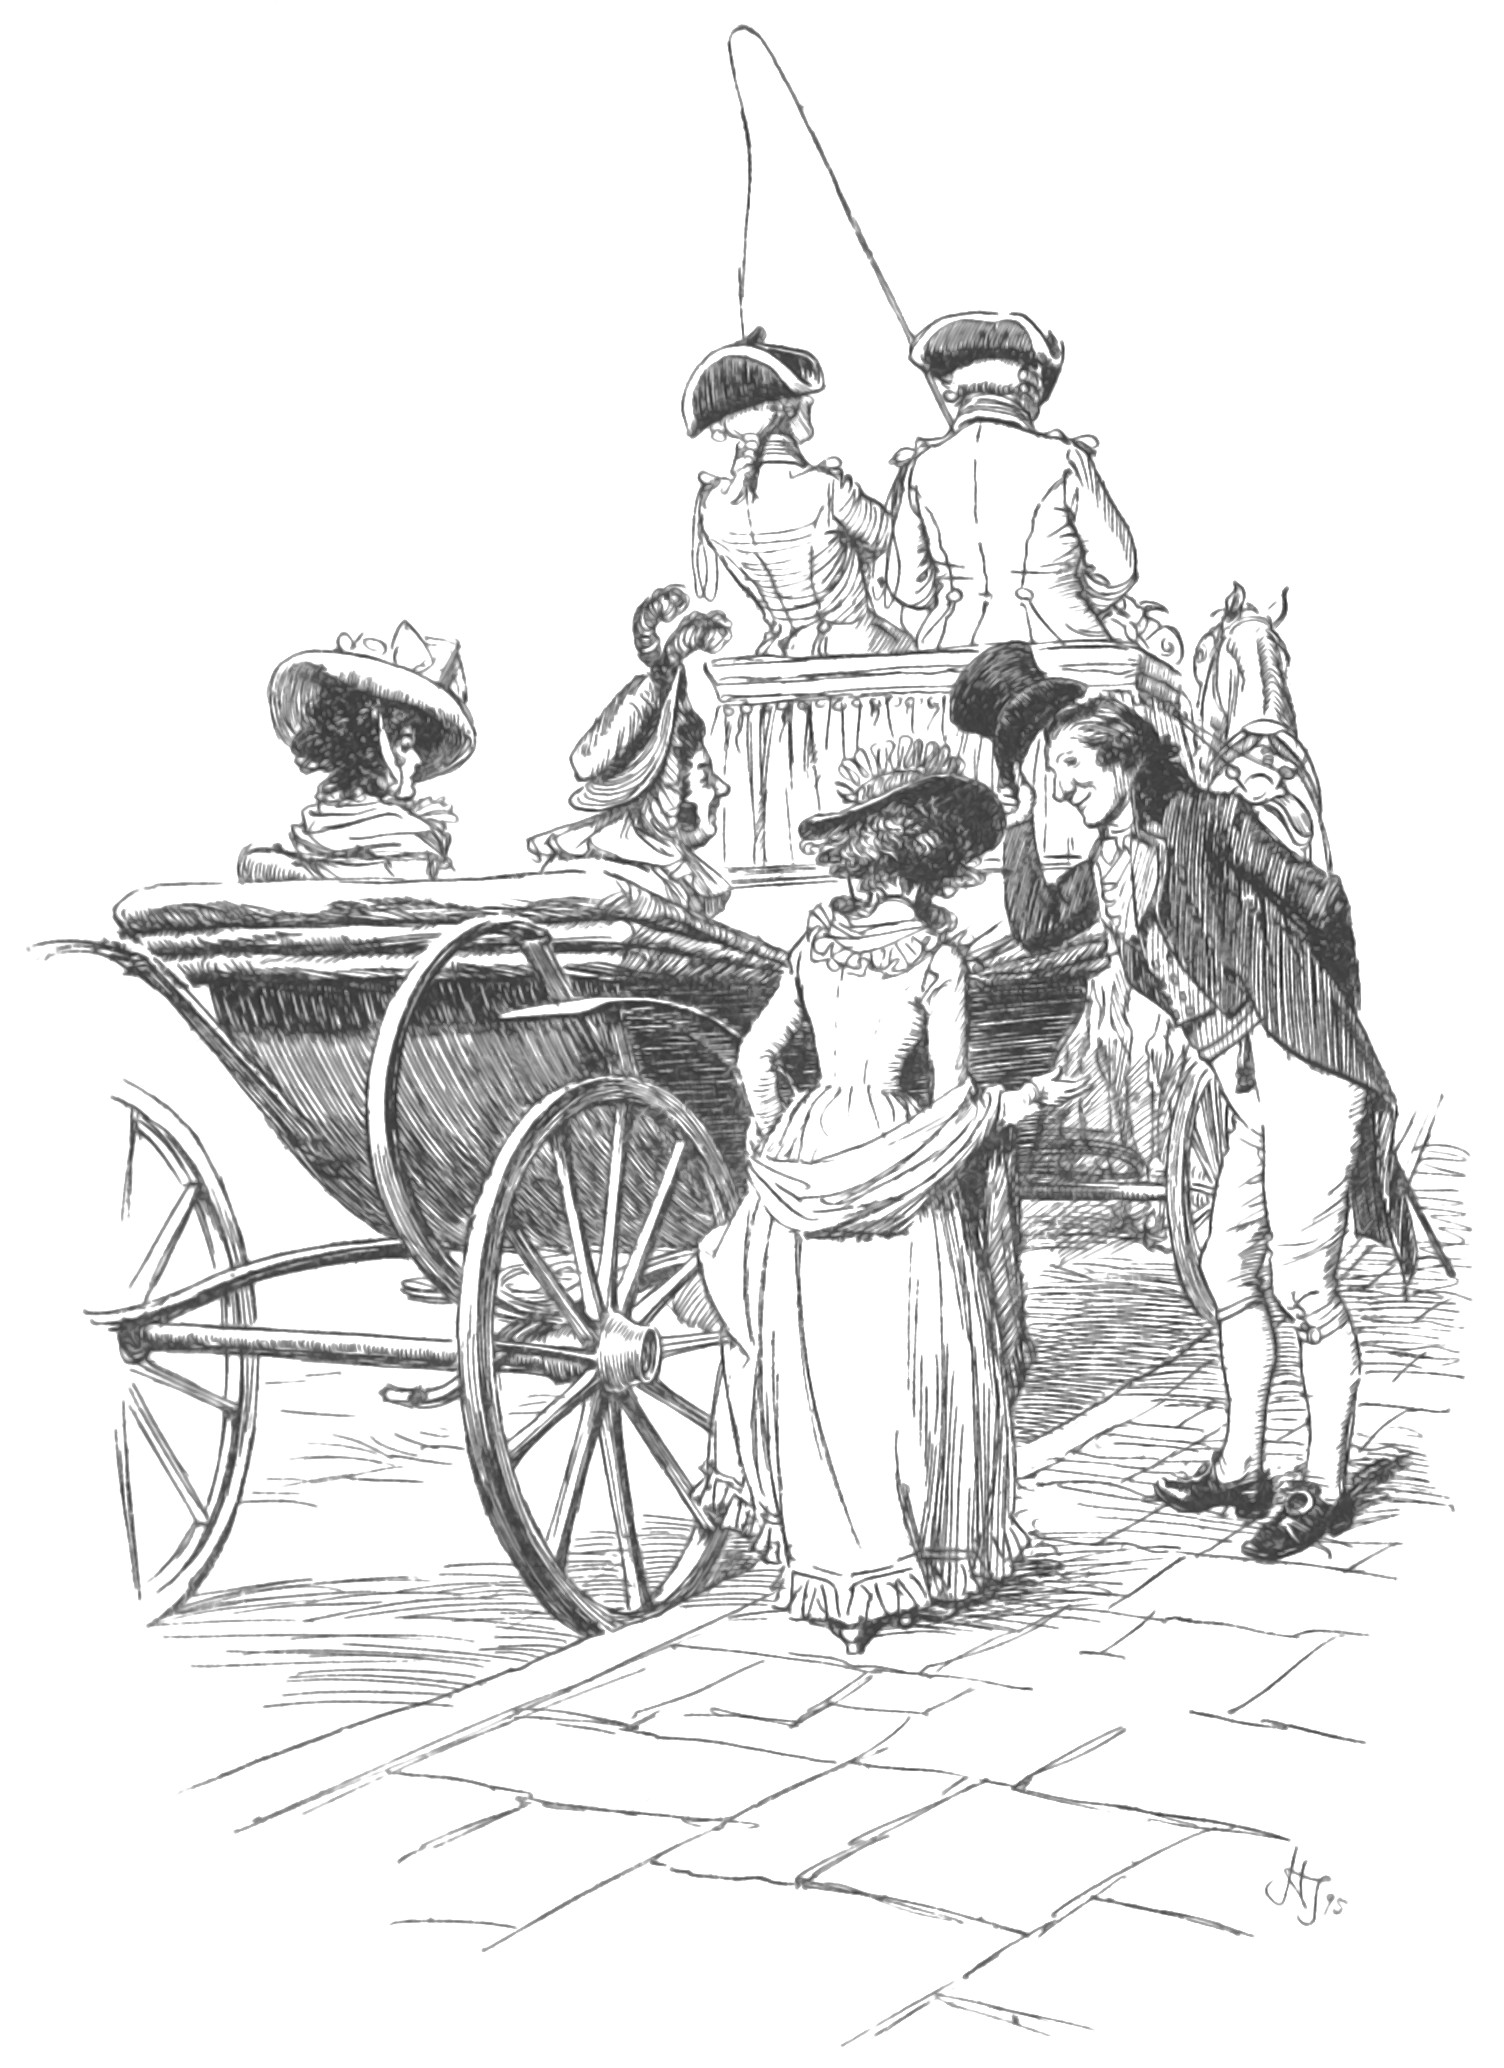
\includegraphics[width=\linewidth]{33introduced}
\caption{Introduced to Mrs Jennings}
\end{figure}

His visit was duly paid. He came with a pretence at an apology from their sister-in-law, for not coming too; <but she was so much engaged with her mother, that really she had no leisure for going any where.> Mrs Jennings, however, assured him directly, that she should not stand upon ceremony, for they were all cousins, or something like it, and she should certainly wait on Mrs John Dashwood very soon, and bring her sisters to see her. His manners to \textit{them}, though calm, were perfectly kind; to Mrs Jennings, most attentively civil; and on Colonel Brandon's coming in soon after himself, he eyed him with a curiosity which seemed to say, that he only wanted to know him to be rich, to be equally civil to \textit{him}.

After staying with them half an hour, he asked Elinor to walk with him to Conduit Street, and introduce him to Sir John and Lady Middleton. The weather was remarkably fine, and she readily consented. As soon as they were out of the house, his enquiries began.

<Who is Colonel Brandon? Is he a man of fortune?>

<Yes; he has very good property in Dorsetshire.>

<I am glad of it. He seems a most gentlemanlike man; and I think, Elinor, I may congratulate you on the prospect of a very respectable establishment in life.>

<Me, brother! what do you mean?>

<He likes you. I observed him narrowly, and am convinced of it. What is the amount of his fortune?>

<I believe about two thousand a year.>

<Two thousand a-year;> and then working himself up to a pitch of enthusiastic generosity, he added, <Elinor, I wish with all my heart it were \textit{twice} as much, for your sake.>

<Indeed I believe you,> replied Elinor; <but I am very sure that Colonel Brandon has not the smallest wish of marrying \textit{me}.>

<You are mistaken, Elinor; you are very much mistaken. A very little trouble on your side secures him. Perhaps just at present he may be undecided; the smallness of your fortune may make him hang back; his friends may all advise him against it. But some of those little attentions and encouragements which ladies can so easily give will fix him, in spite of himself. And there can be no reason why you should not try for him. It is not to be supposed that any prior attachment on your side—in short, you know as to an attachment of that kind, it is quite out of the question, the objections are insurmountable—you have too much sense not to see all that. Colonel Brandon must be the man; and no civility shall be wanting on my part to make him pleased with you and your family. It is a match that must give universal satisfaction. In short, it is a kind of thing that>—lowering his voice to an important whisper—<will be exceedingly welcome to \textit{all parties}.> Recollecting himself, however, he added, <That is, I mean to say—your friends are all truly anxious to see you well settled; Fanny particularly, for she has your interest very much at heart, I assure you. And her mother too, Mrs Ferrars, a very good-natured woman, I am sure it would give her great pleasure; she said as much the other day.>

\begin{figure}[tbph]
\centering

\includegraphics[width=\linewidth]{33assured}
\caption{Mrs Jennings assured him directly}
\end{figure}

Elinor would not vouchsafe any answer.

<It would be something remarkable, now,> he continued, <something droll, if Fanny should have a brother and I a sister settling at the same time. And yet it is not very unlikely.>

<Is Mr Edward Ferrars,> said Elinor, with resolution, <going to be married?>

<It is not actually settled, but there is such a thing in agitation. He has a most excellent mother. Mrs Ferrars, with the utmost liberality, will come forward, and settle on him a thousand a year, if the match takes place. The lady is the Hon. Miss Morton, only daughter of the late Lord Morton, with thirty thousand pounds. A very desirable connection on both sides, and I have not a doubt of its taking place in time. A thousand a-year is a great deal for a mother to give away, to make over for ever; but Mrs Ferrars has a noble spirit. To give you another instance of her liberality:—The other day, as soon as we came to town, aware that money could not be very plenty with us just now, she put bank-notes into Fanny's hands to the amount of two hundred pounds. And extremely acceptable it is, for we must live at a great expense while we are here.>

He paused for her assent and compassion; and she forced herself to say,

<Your expenses both in town and country must certainly be considerable; but your income is a large one.>

<Not so large, I dare say, as many people suppose. I do not mean to complain, however; it is undoubtedly a comfortable one, and I hope will in time be better. The enclosure of Norland Common, now carrying on, is a most serious drain. And then I have made a little purchase within this half year; East Kingham Farm, you must remember the place, where old Gibson used to live. The land was so very desirable for me in every respect, so immediately adjoining my own property, that I felt it my duty to buy it. I could not have answered it to my conscience to let it fall into any other hands. A man must pay for his convenience; and it \textit{has} cost me a vast deal of money.>

<More than you think it really and intrinsically worth.>

<Why, I hope not that. I might have sold it again, the next day, for more than I gave: but, with regard to the purchase-money, I might have been very unfortunate indeed; for the stocks were at that time so low, that if I had not happened to have the necessary sum in my banker's hands, I must have sold out to very great loss.>

Elinor could only smile.

<Other great and inevitable expenses too we have had on first coming to Norland. Our respected father, as you well know, bequeathed all the Stanhill effects that remained at Norland (and very valuable they were) to your mother. Far be it from me to repine at his doing so; he had an undoubted right to dispose of his own property as he chose, but, in consequence of it, we have been obliged to make large purchases of linen, china, \&c. to supply the place of what was taken away. You may guess, after all these expenses, how very far we must be from being rich, and how acceptable Mrs Ferrars's kindness is.>

<Certainly,> said Elinor; <and assisted by her liberality, I hope you may yet live to be in easy circumstances.>

<Another year or two may do much towards it,> he gravely replied; <but however there is still a great deal to be done. There is not a stone laid of Fanny's green-house, and nothing but the plan of the flower-garden marked out.>

<Where is the green-house to be?>

<Upon the knoll behind the house. The old walnut trees are all come down to make room for it. It will be a very fine object from many parts of the park, and the flower-garden will slope down just before it, and be exceedingly pretty. We have cleared away all the old thorns that grew in patches over the brow.>

Elinor kept her concern and her censure to herself; and was very thankful that Marianne was not present, to share the provocation.

Having now said enough to make his poverty clear, and to do away the necessity of buying a pair of ear-rings for each of his sisters, in his next visit at Gray's, his thoughts took a cheerfuller turn, and he began to congratulate Elinor on having such a friend as Mrs Jennings.

<She seems a most valuable woman indeed. Her house, her style of living, all bespeak an exceeding good income; and it is an acquaintance that has not only been of great use to you hitherto, but in the end may prove materially advantageous. Her inviting you to town is certainly a vast thing in your favour; and indeed, it speaks altogether so great a regard for you, that in all probability when she dies you will not be forgotten. She must have a great deal to leave.>

<Nothing at all, I should rather suppose; for she has only her jointure, which will descend to her children.>

<But it is not to be imagined that she lives up to her income. Few people of common prudence will do \textit{that} and whatever she saves, she will be able to dispose of.>

<And do you not think it more likely that she should leave it to her daughters, than to us?>

<Her daughters are both exceedingly well married, and therefore I cannot perceive the necessity of her remembering them farther. Whereas, in my opinion, by her taking so much notice of you, and treating you in this kind of way, she has given you a sort of claim on her future consideration, which a conscientious woman would not disregard. Nothing can be kinder than her behaviour; and she can hardly do all this, without being aware of the expectation it raises.>

<But she raises none in those most concerned. Indeed, brother, your anxiety for our welfare and prosperity carries you too far.>

<Why, to be sure,> said he, seeming to recollect himself, <people have little, have very little in their power. But, my dear Elinor, what is the matter with Marianne?—she looks very unwell, has lost her colour, and is grown quite thin. Is she ill?>

<She is not well, she has had a nervous complaint on her for several weeks.>

<I am sorry for that. At her time of life, any thing of an illness destroys the bloom for ever! Hers has been a very short one! She was as handsome a girl last September, as I ever saw; and as likely to attract the man. There was something in her style of beauty, to please them particularly. I remember Fanny used to say that she would marry sooner and better than you did; not but what she is exceedingly fond of \textit{you}, but so it happened to strike her. She will be mistaken, however. I question whether Marianne \textit{now}, will marry a man worth more than five or six hundred a-year, at the utmost, and I am very much deceived if \textit{you} do not do better. Dorsetshire! I know very little of Dorsetshire; but, my dear Elinor, I shall be exceedingly glad to know more of it; and I think I can answer for your having Fanny and myself among the earliest and best pleased of your visitors.>

Elinor tried very seriously to convince him that there was no likelihood of her marrying Colonel Brandon; but it was an expectation of too much pleasure to himself to be relinquished, and he was really resolved on seeking an intimacy with that gentleman, and promoting the marriage by every possible attention. He had just compunction enough for having done nothing for his sisters himself, to be exceedingly anxious that everybody else should do a great deal; and an offer from Colonel Brandon, or a legacy from Mrs Jennings, was the easiest means of atoning for his own neglect.

They were lucky enough to find Lady Middleton at home, and Sir John came in before their visit ended. Abundance of civilities passed on all sides. Sir John was ready to like anybody, and though Mr Dashwood did not seem to know much about horses, he soon set him down as a very good-natured fellow: while Lady Middleton saw enough of fashion in his appearance to think his acquaintance worth having; and Mr Dashwood went away delighted with both.

<I shall have a charming account to carry to Fanny,> said he, as he walked back with his sister. <Lady Middleton is really a most elegant woman! Such a woman as I am sure Fanny will be glad to know. And Mrs Jennings too, an exceedingly well-behaved woman, though not so elegant as her daughter. Your sister need not have any scruple even of visiting \textit{her}, which, to say the truth, has been a little the case, and very naturally; for we only knew that Mrs Jennings was the widow of a man who had got all his money in a low way; and Fanny and Mrs Ferrars were both strongly prepossessed, that neither she nor her daughters were such kind of women as Fanny would like to associate with. But now I can carry her a most satisfactory account of both.>